\section{Preface}
This chapter was published in the Proceedings of the ACM Conference on Human Factors in Computing Systems in May 2017. It was titled ``Disempowered by Data:  Nonprofits, Social Enterprises,and the Consequences of Data-Driven Work'', and was co-authored with Ellie Harmon and Amy Voida (author order was Bopp, Harmon, Voida). It is included here as published with the permission of my co-authors.

\section{Introduction}
In the move toward rationalization and quantification in organizations \citep{Morgan1997Images}, the increasing prevalence of information systems designed to support the collection, management, and analysis of data has coincided with expectations that organizations should be more “data-driven”---using increasingly larger aggregations of data to enable more productive and empowered decisions. Previous research in the management of information systems has suggested that, in for-profit contexts, data-driven decision making leads to improvements in performance, output, and productivity \citep{Brynjolfsson2011Strength,Lavalle2011Big}. In the nonprofit context, data-driven decision making has been shown to improve “the effectiveness of management decisions” \citep{Maxwell2016Data} (see also \citep{Leroux2010Does}). Yet scholarship about data and its impacts on organizations in HCI and adjacent fields has raised critical concerns about this “march toward quantification” \citep{Lohr2012Age}---concerns about the ways in which the quantification of data changes assumptions about the meaning of knowledge and about how people “should” engage with information, concerns about the biases inherent in and the decontextualization of big data, and concerns about the new digital divides created by big data \citep{Boyd2012Critical,Pine2015Emerging,Punathambekar2015Debating}.

Recent empirical research has also raised significant concerns about how “cultures of data” are enacted in organizations \citep{Verma2016DrillDown}. This research has identified significant disconnects between the support provided by collaborative computing systems and the organizational practices that are developing in response to calls for organizations to become more data-driven. In addition, questions remain about how work practices and organizational identity are shaped by the expectations and demands of being data-driven \citep{Pine2015Emerging,Power1997Audit,Pentland2000Auditors}.

In this research, we expand on this nascent but growing body of empirical work by examining the enactment---and consequences---of monitoring and evaluation (M\&E) in mission-driven organizations. Encompassing nonprofit organizations and social enterprises, mission-driven organizations differ from traditional for-profit corporations in that organizational goals are rooted in social impact, rather than solely in profit-based bottom lines.

Research about the uptake of data-driven practices in the mission-driven context is critical as recent investigations have raised concerns over the efficacy of data practices in mission-driven organizations. Maxwell et al. found that in social enterprise organizations, “data are often collected but less often analyzed” \citep{Maxwell2016Data}. And although individuals in these organizations believed in the potential of data-driven decision making, they reported “less confidence in their organization’s ability to do so” \citep{Maxwell2016Data}. 

In this paper, we present findings from an empirical study of the use of data in 13 mission-driven organizations. Drawing on interviews with 19 M\&E professionals, we find critical consequences in how data practices are emerging in these organizations. The mission-driven organizations that participated in this research are not empowered by data. Instead, they are investing time, sacrificing expertise, and responding to largely external demands for data collection and reporting at the expense of the mission and operation of the organization. We identify three negative consequences of current data practices---\textit{erosion of autonomy, data drift, and data fragmentation}---which are mutually reinforcing and lead to a cycle of increasing disempowerment. This \textit{cycle of disempowerment} results in organizations having less control over their own data practices—preventing the meaningful use of data and discouraging the organization from redesigning data practices to better meet their needs.

\section{Related Work}
\subsection{Data-Driven Practices}

Researchers have identified many benefits of using technology for data-driven practices, including the optimization of production and manufacturing, reductions in customer attrition, reductions in data redundancy, facilitation of new genres of questions by end-users, increased profitability, and the creation of competitive advantage \citep{Kohavi2002Trends,Piccoli2008Profit,Watson2007Current}. When these tools are successfully leveraged for data-driven decision making, these practices are found to improve performance, productivity, and effectiveness \citep{Brynjolfsson2011Strength,Lavalle2011Big,Leroux2010Does}.

Yet, previous research has also raised concerns about the biases of big data leading to new digital divides between data-haves and have-nots and between individuals and organizations that do and do not have computational literacies \citep{Boyd2012Critical,Kitchin2014Big,Manovich2011Trending}. Manovich suggests that big data has created new inequalities among three categories of people and organizations: “those who create data (both consciously and by leaving digital footprints), those who have the means to collect it, and those who have expertise to analyze it.” \citep{Manovich2011Trending}

boyd and Crawford suggest that two digital divides fall out of these inequalities: one related to who does and does not have access to big data and a second related to who does and does not have the ability to \textit{utilize} this data \citep{Boyd2012Critical}. Concerns about the uneven uptake of big data become even more critical as the purview of data-driven practices are expanding beyond the private sector. As King asserts:

\begin{quote}\singlespacing The march of quantification, made possible by enormous new sources of data, will sweep through academia, business and government. There is no area that is going to be untouched (quoted in \citep{Lohr2012Age}; see also \citep{Brynjolfsson2011Boom,Kitchin2014Big}).\end{quote}

It becomes increasingly important, then, to understand the ways in which data-driven practices are taken up or attempted in a diversity of organizational contexts.

\subsection{Data in the Nonprofit Sector}
Nearly all research exploring the role of technology in the nonprofit sector highlights the extraordinary constraints in resources and expertise that shape the way systems are and are not used (e.g., \cite{Merkel2007Learning,Voida2011Homebrew}). Information management, in particular, is a challenge for these organizations. Voida et al. have characterized the patchwork assemblages of information systems in the nonprofit sector as “homebrew databases” \citep{Voida2011Homebrew}. Working within the myriad of constraints in these organizations, individual knowledge workers creatively appropriate disparate paper tools, personal information management systems, and---sometimes---enterprise or custom databases to satisfice their data practices. But these “homebrew databases” are plagued with significant version control issues, redundant data entry, a lack of scalability, siloed and/or inaccessible data, an unproductive churn through the adoption and use of different tools, and, ultimately, an abandonment of data. 

These challenges are not solved in even the leading edge organizations in the sector. Verma and Voida’s case study of one such organization’s adoption of a business intelligence system also found pervasive challenges in data warehousing \citep{Verma2016DrillDown}. Much of the organization’s data was siloed in systems for which there was no import mechanism; some data was kept in spreadsheets and had to be manually updated daily; and some data was not digitized at all. 

All of these issues make engaging in data analysis a nearly intractable problem. Perhaps it is unsurprising, then, that a survey of the capacity for data-driven decision making in social enterprise organizations found that while organizations are collecting a large quantity of data, they are not adept or confident about analyzing or using that data \citep{Maxwell2016Data}. 

Supporting information management in the nonprofit sector is particularly important as these organizations are under increasing pressure to provide impact and performance data to funders \citep{Haskins2011Building}. Yet, Snibbe warns of the costs: “Nonprofits are often collecting heaps of dubious data, at great cost to themselves and ultimately to the people they serve” \citep{Snibbe2006Drown}. Indeed, research in philanthropic studies cautions that many of the performance metrics used in nonprofit organizations fail to account for critical aspects of nonprofit work and, in fact, might be impeding performance \citep{Benjamin2014Programs}. Understanding the role of data in the work of mission-driven organizations will be critical to better supporting and empowering these organizations.

\section{Methods}
\subsection{Participants}

We recruited 19 participants (referenced by an anonymous participant number, P1–P19) from 13 mission-driven organizations, all of whom were responsible for some aspect of the monitoring and evaluation (M\&E) work in their organization. M\&E professionals typically serve as the central points of expertise regarding data in their organization, often responsible for operationalizing and carrying out requests for data—whether originating inside or outside the organization. As such, these individuals offer a uniquely broad perspective about how data is taken up and used---and the implications of that use---across the organization. We recruited participants initially through snowball sampling, starting with M\&E professionals who participated in a community professional development event. As our research unfolded, we engaged in theoretical sampling, strategically recruiting from additional organizations to obtain diversity on two dimensions: type of organization and annual revenue.

We sampled from three types of mission-driven organizations to create maximum variation:

\begin{enumerate}
\item Direct service nonprofit organizations provide a variety of services to clients (n=9 participants from 8 organizations);
\item Indirect service nonprofit organizations provide services to other nonprofit organizations, including research services and funding (n=9 participants from 4 organizations); and
\item Social enterprises are mission-driven, for-profit organizations or programs within nonprofit organizations (n=1 participant from 1 for-profit social enterprise, plus n=8 participants already included above from 6 nonprofit organizations who manage social enterprise programs).
\end{enumerate}

We also sampled across a range of organizations’ annual revenue. Because data practices are often prescribed by funders, we consider a range of annual revenues to signify a range of experiences with data practices. Organizations sampled ranged in annual revenue from \$100K to \$75M. Within these annual revenue figures we, once again, used available data to sample across predominant revenue sources: government grants, membership dues, fundraising events, program service revenue, and sale of inventory.

\subsection{Data Collection}
We collected data through semi-structured interviews using an interview protocol that focused on three areas of inquiry: (1) the nature of the participant’s work within and/or alongside other mission-driven organizations, (2) the role of data and related technologies in the participants’ work, and (3) the organizations’ approaches to impact measurement including the types of data collected and the information systems leveraged. The first author conducted all interviews and adapted the interview protocol based on grounded theory’s principle of constant comparison to gather “additional data samples that are chosen to test the theory at its weakest point” \citep{Muller2014Grounded}. One interview question, for example began broadly as ‘How and why do you collect data on your organization’s programs?’ and evolved into a request, for each type of data, for the participant to ‘tell [us] more about who the audience is and how that audience shaped the process.’ This evolution was driven by accounts of power and influence offered by early study participants and was designed to better understand how external audiences were or were not involved in the day-to-day operational decisions of data collection and at what level of specificity.

Interviews lasted on average 56 minutes. The majority of the interviews were conducted within a one month period, with additional interviews conducted several months later after preliminary data analysis. We audiotaped and transcribed each interview to aid in analysis.

\subsection{Data Analysis}
We took an inductive approach to data analysis (following \cite{Corbin2014Basics}), grounded in coding and memoing techniques. We identified emergent themes such as evaluative approaches, organizational constraints, and technical capacity through open coding. We printed, cut up, and clustered the coded transcripts to develop axial codes that surfaced themes about the relationship between organizations’ internal capacities, externally imposed constraints, and data complexity.

We interleaved the second stage of analysis with additional data collection, using our axial codes to “interrogate the open codes, leading to more data collection and more open coding” \citep{Muller2014Grounded}. We then engaged in several iterations of affinity diagramming to identify cross-cutting categories that allowed us to make sense of participants’ experiences and understandings of M\&E work in mission-driven organizations. We tested each at its weakest point through memos and discussions among researchers, frequently returning to the transcripts as reference. This multi-stage analytic process resulted in the identification of three key consequences of monitoring and evaluation. In subsequent theoretical integration, we explored the interrelationships among these consequences, leading us to propose a \textit{cycle of disempowerment} for mission-driven organizations.

\subsection{Methodological Limitations}
Grounded theory---and all research methods—include many trade---offs in the kinds of evidence they generate and the kinds of conclusions and theory building they facilitate. An interview-based grounded theory approach is well suited to this research as we sought to understand the practices, experiences, and implications of data in mission-driven organizations. This approach offers opportunities for what \cite{Lincoln1985Naturalistic} refer to as “transferability”---the evidence-based argument that analytical insights are applicable beyond the specific individuals studied. This affordance of qualitative methods is enabled by strategies such as constant comparison rather than being rooted in ideals of statistical generalizability or bias-free objectivity \citep{Lincoln1985Naturalistic}.

\subsection{Research Context: Monitoring \& Evaluation in Mission Driven Organizations}
Mission-driven organizations are entities, both large and small, for-profit and not-for-profit, that aim to have a particular impact on society as described by their organizational mission. Generally, this mission is geared toward having an effect on one or more critical issues facing society, such as health or education. For the purpose of this study, organizations were considered mission-driven if they were either a traditional nonprofit organization or a social enterprise that placed the importance of social impact at an equal or greater level than profit.

The hub of data collection and use within mission driven organizations is the monitoring and evaluation (M\&E) department or, more likely, a singular M\&E professional who may also have several other job responsibilities. The individual(s) responsible for M\&E oversee the on-going monitoring of program activities against targeted outputs and outcomes. They also may conduct more comprehensive retrospective evaluations that examine the program’s operation and assess progress towards intended short-term and long-term outcomes. This work often involves orienting to an organizational “theory of change,” a model that (a) represents how a social intervention intends to use resources to perform programmatic activities and ultimately achieve the desired social impact, and (b) suggests specific metrics that the organization should be using to measure impact.

The unique mission-driven context shapes organizations’ relationships to data, impacts how that data can ultimately be put to use, and influences to what ends and for whom it can serve. To situate the findings of this work, we first provide some background on four key characteristics of the mission-driven context: limited resources, grant-driven business models, social impact measurement, and reliance on external experts. Each characteristic is well-established in nonprofit management but where appropriate, we augment our characterization with specific references to participants in this study to illustrate more concretely how these characteristics influence data practices.

\subsubsection{Limited Resources}
The experiences of participants in this research confirm prior findings that nonprofits have limited financial and labor resources (e.g., \cite{Merkel2007Learning,Voida2011Homebrew}). These limitations influence data practices from collection to analysis to reporting. Participants were particularly attuned to the limitations of time as a resource, and framed many of their frustrations in terms of having to make difficult tradeoffs as a result. Often, organizations restrict the time spent on data practices to that which is obligated by external funders. So while significant time is devoted to collecting data, analyzing that data beyond the production of reports for external funders is rare.

\subsubsection{Grant-Driven Business Model}
The organizations in this research were all, to varying degrees, reliant on grants made by external funding agencies to carry out their work. This means that funders have significant sway over organizations, which we see manifesting through prescriptions about what data to collect, how to report on it and how to interpret it. Organizations with funding from multiple sources had to negotiate compounding—and sometimes conflicting—requirements for data collection, management, and reporting. This can be problematic because it amplifies an existing challenge that arises from a misalignment of goals between funding bodies and the organizations themselves.

\subsubsection{Social Impact Measurement}
Mission-driven organizations try to intervene in complex, large-scale social issues that make both data collection and analysis difficult. Any change caused by the work of the organization is intertwined with—and likely indistinguishable from—the variety of other social changes happening concurrently: ranging from changes in government programs, to local economic shifts, to even more localized changes within the lives of families and individuals served by organizations. Organizational “impact” is not easily disentangled or isolated in ways that may be attributed causally to a particular program. 

Complicating the difficulties of establishing causality, social impact is something that cannot be achieved overnight---it takes time. This means that data collection must be longitudinal in order to be most useful. Yet, knowing what data to collect at the start of a program is often impossible. Consequently, datasets collected by organizations are often incomplete---beginning with one set of metrics, and shifting over time to include more or simply different metrics. 

\subsubsection{Reliance on External Experts}
Similar to the findings of Erete et al that described nonprofits’ reliance on external experts for “open data” work \citep{Erete2016Storytelling}, we found that M\&E data practices are also generally reliant on external experts. For the organizations in this study, external experts included: professional evaluators, researchers, graduate student interns, data scientists, regional coordinators, and technology consultants. M\&E professionals have expectations about the differing abilities of each group, with volunteer data scientists providing “game changing” assistance and interns providing hit-or-miss help. Yet, in the case of smaller, more resource-constrained organizations, unpaid interns are the only realistic option. Organizations with more financial resources were more likely to have a dedicated “data analyst” on staff, however, even in these cases professional consultants are still hired on a temporary basis. Despite differing levels of knowledge and experience, our participants generally felt that all of these experts have the necessary expertise to be able to work with the intricacies of their data. 

\section{Findings}
We find that mission-driven organizations’ monitoring and evaluation (M\&E) practices result in three unforeseen and negative consequences that are mutually reinforcing and lead to a cycle of increasing disempowerment for the organization. These consequences are: \textit{erosion of autonomy, data drift, and data fragmentation}.

\subsection{Erosion of Autonomy}
All participants described experiencing an \textit{erosion of autonomy}---including individual and organizational autonomy---over data practices due to the influence of external actors, including funding bodies, boards, ratings agencies, and information technologies. This array of actors exerts influence, impinging upon organizations’ autonomy in making decisions about choosing metrics, compiling and using data, and prioritizing data work.

\subsubsection{Choosing Metrics}
Before decisions about data use could be made, participants’ accounts suggest that external actors wore away at organizations’ autonomy in making choices about what data should be collected and what metrics should be computed. P8, for example, described getting...

\begin{quote}\singlespacing...caught up in reporting the indicators that are required to the people that are paying the bills rather than necessarily taking space to step back and look at the whole picture. (P8)\end{quote}

Compounding long-standing requirements of funding bodies for certain data---e.g. beneficiary demographic data, or output metrics like number of people served---external groups are asking for additional, more specific, data. One participant described the recent actions of a rating agency: “They’re trying to have organizations fill out [forms to answer the question of] how do you know what you’re doing makes a difference?” (P3)

Though rating agencies have historically relied on data from tax forms, a participant who worked for a nonprofit organization that assigns ratings to other nonprofits affirmed that agencies are increasingly asking organizations to provide additional data, particularly impact data: “If you want to get your 4-star rating, you’re going to have to be talking about how you’re tracking impact” (P4). Similarly, another participant speaks about funders:

\begin{quote}\singlespacing 20 years ago, output data was really the only thing we had and that’s all people asked for, was, you know, how many people did you serve? Well now, for sophisticated funders, that’s not enough. (P14)\end{quote}

\subsubsection{Compiling and Using Data}
When it comes to making decisions about how to operationalize measures like impact, organizations in this study were not only pressured about what data to collect, but also about what \textit{kind} of data to use for what purpose. Board members wanted to market “feel good” (P12) stories informally obtained outside of the evaluation process:

\begin{quote}\singlespacing Our board...they get real hung up on the marketing story instead of, well, what's the evidence for the marketing story? I've introduced this phrase \textit{evidence-based marketing metrics} to them, but it's kind of a struggle. I would like this [evaluation] data to be used for board and fundraisers to be able to have some real things to report on instead of 'Oh, it's all so great!' (P12)\end{quote}

Board members further shaped organizations’ data practices through constraints about how data should be reported. In our participants’ experiences, board members are more interested in looking at executive summaries of data analysis---more conducive to glance-able graphs or a “feel good” quote, not details of nuanced analyses.

As organizations move towards computational systems of measurement, they are also encountering information systems that prioritize quantitative over qualitative forms of data. As P10 explained about her organization’s database: “We would need to have people answer qualitative questions in a quantitative way. So, ‘how did this make you feel on a scale of 1 to 10?’” (P10) 

Even at the funder level, information systems served to steer staff members towards quantitative data that can more easily be accessed and queried. This was explained by a staff member at a community foundation:

\begin{quote}\singlespacing Any reporting...[on] the difference we made in the community...is outside of any formal IT system. It’s coming in probably on a dozen different channels, with a dozen different formats and it’s not centralized. So, if someone were to say I need to measure our impact, [the IT systems] wouldn’t be very much help. [Using the database], I could tell them where the money went...[but] if you want to know the stories...about what difference we made, you need to go talk to [a program staff member] because I don’t have anything I can touch that gets to that. (P16)\end{quote}

In addition to these constraints on what data to collect and what kinds of data are considered valuable, participants’ accounts suggests that decisions about how to use data were further sites of eroded autonomy. There is a key distinction between the evaluation work required by funders and a more rigorous evaluation that would more closely benefit the mission of the organization. Often, evaluation work required by grants, referred to as “implementation evaluation” by P15, is not intended to understand how a program has caused a change in society, instead it is intended to determine if the grant dollars were spent in the agreed upon manner.

\begin{quote}\singlespacing Funders are interested in building evaluation in around the specific objectives of that project...It’s more of an implementation research question that funders have...Really rigorous evaluation of what works...that’s the type of evaluation that it’s harder to get a funder to say ‘Oh yeah, I’ll do that.’ For instance, we have a couple projects where...we have a comparison group that we’re working with that isn’t getting the intervention. That type of project is expensive, and funders have to have the vision to see that what we’ll learn from that might have a lot of later potential impact if we know if the intervention works. (P15)\end{quote}

When broader social impacts are valued, report preparation timelines can prohibit longer term evaluations as granting agencies operate on short-term cycles (and thereby encourage surface level evaluation) rather than asking for or rewarding in-depth and longitudinal evaluation. Moreover, participants reported challenges in putting reports to use internally which had been prepared for the primary consumption of external stakeholders. For P10, it is challenging to resist the option of “just taking the report and putting it on the shelf” (P10). Even though a report might contain potentially useful data about operations, leveraging the report in ways that might inform internal practices would require additional time that staff do not have. 

\subsubsection{Prioritizing Data Work}
The many data collection requirements and the use of data by external actors to evaluate and rate mission-driven organizations contribute to eroding organizations’ autonomy over their own processes. This occurs at the most mundane and micromanaging kind of level: how to prioritize staff time. Staff members in this study reported a lack of time to accomplish their many tasks which often resulted in a prioritization of data work for funders over that which might be done for the organization. One participant explained: “Taking all of that data, entering it into something that makes it make sense, and figuring out how to use it is never a priority when there are fires to put out every day” (P8). Despite these fires, P8 finds time to collect and report on indicators that the funders want.

The kinds of rigorous evaluations that participants report would allow organizations to examine their own programs in terms of long-term causal outcomes are not supported within the rubric of most grants, the data demands of ratings agencies, or the information systems designed for tracking and analyzing only limited kinds of metrics. Funding for additional data work is harder to find in the mission-driven environment, which is increasingly dominated by directed funding earmarked for specific programs. Initiatives to build organizational capacity and infrastructure for data work---often referred to as “administrative overhead”---weighs against an organization’s perceived effectiveness and efficiency in carrying out their mission.

When data collection must conform to frameworks and blueprints dictated by funders, organizations are left juggling everyone’s needs except their own. The accounts of data work reflected by participants suggests that organizations are operating within a cacophony of data strategies. Regardless of who is setting the direction and what their motivation is, choices about what data to collect and report are partially driven by whomever happens to be providing direction. In this diverse ecosystem of data stakeholders, it is unclear that there is ever a single, overarching plan. What is clear, however, is that the organizations, themselves, have relatively little autonomy in setting or even providing input into that overarching plan---which lays a foundation for organizational disempowerment.

\subsection{Data Drift}
The nonprofit sector refers to the move away from an organization’s mission over time as “mission drift” \citep{Moore2000Managing}. Mission drift has severely negative connotations as organizations are involuntarily and unknowingly pulled away from their original mission toward a new one. In our research, we see a similar shift at the level of data. Through \textit{data drift}, organizations change the kind of metrics that they collect and manage over time as their organizational identity, as represented by data, evolves. Despite the possibility that an approach to M\&E may not be a good match for the organization, an eroding autonomy can prevent them from putting their data trajectory back on course. As misguided data is used in evaluation and funding decisions, the next round of data collection requirements are likely to be even further from the organization’s intended direction.

For the participants in this study, external influences cause \textit{data drift} at multiple stages of the organization’s workflow: from initial, orienting theories of change to final reporting. For example, one participant (P11) described how the organization’s theory of change was developed not from rigorous research or impact measurement, but rather based on the \textit{funder’s} objectives by “scoping and identifying” where their project had the most demonstrable impact. In this instance, the funder was comparatively hands-off, yet still indirectly manipulated the way that staff viewed their program’s impact. Theories of change influence choices of what indicators to track, and defining change rooted in funders’ objectives leads to shifts in data collection towards the funder’s priorities, all the while neglecting metrics more squarely related to the organization’s own mission.

In another instance, one executive director (P8) explained that she sees her organization as helping individuals escape poverty. However, one of their two primary funders is particularly interested in their work in terms of its environmental impact---because that is the funder’s mission. From the nonprofit’s perspective, they feel that their program’s environmental impact is “nothing” compared to other renewable energy projects. However, the funder is “very interested in those environmental indicators, and so we end up doing a lot of weird environmental stuff that we don’t typically focus on” (P8). Thus, \textit{data drift} is perpetuated in this organization because of their ambivalence about pushing back on a “strong” funder. P8 continues by describing how funders shape data collection decisions:

\begin{quote}\singlespacing We find ourselves kind of hustling to do M\&E in a way that might not necessarily always make sense for us. But we need it for a report, and we need these numbers and even if it’s something that we’ve never thought about collecting before, it’s like, well, figure out how to collect it because so and so says we need it. (P8)\end{quote}

P8 goes on to describe how grant-based funding can impact the mission of the organization over time:

\begin{quote}\singlespacing [It is] not a very sustainable way to ensure effective sustainable growth... It’s really hard to find the perfect fit grant that allows you to just keep doing what it is that you know your organization does best. Because you then end up tied to... the indicators or the activities... as dictated by what your funder wants to see. (P8)\end{quote}

This reflection suggests that \textit{data drift} may function as a precursor to mission drift. As data is collected in accordance with the funder’s desires, the organization may shift focus, further contributing to organizational disempowerment.

\subsection{Data Fragmentation}

Compounding this situation of \textit{data drift}, funders struggle to determine what data they should require from organizations in the first place. This lack of clarity at the funder level, coupled with the fact that many organizations are juggling the demands of multiple funders---a complicated puzzle that organizations must negotiate with their limited resources---results in an accumulation of fragmented data sets. Numerous participants reported being plagued by a proliferation of data that were not connected to each other in any systematic way, creating difficulties for performing social impact measurement. The resulting fractured and incoherent set of data is hard to analyze or put to any kind of use. Thus, while participants reported “swimming in data” (P15), the lack of a systematic data plan from the organization’s point of view limits and constrains the usefulness and impact of data, leading to further organizational disempowerment. The \textit{data fragmentation} reported by participants is multi-faceted. It is fragmented locationally, logically, and longitudinally.

\subsubsection{Locational Fragmentation}
Locational fragmentation occurs when different data are in different systems. For two participants, locational fragmentation resulted from a lack of funding that prevented them from accessing a single, centralized enterprise-level data management system. Instead, in both of these cases, participants’ leveraged multiple, free cloud services for storing data. As P11 explained, data management is particularly difficult “across a team... who don’t have a lot of money to invest in cloud services besides Dropbox and Google” (P11).

Such cases of locational fragmentation were a frequent source of confusion (see also \citep{Voida2013Turbulence}) at another organization:

\begin{quote}\singlespacing [There is not] one place where we can have everything, it’s like OK well you have Google Drive, and some people use Dropbox and some people use our database... it’s really confusing to be like well where was that data stored?... [I received] an invitation for Dropbox stuff a couple days ago. It’s like ahh, I forgot we were using that for stuff, for some reason, I don’t know why we were—probably ran out of room on Google Drive so they started using something else. (P7)\end{quote}

In addition to this locational fragmentation that occurs within individual organizations, locational fragmentation also occurs across organizational boundaries. All participants in this research discussed sharing data with external parties and relying on others to share relevant data in return. Yet, this sharing of data across organizations was not always easy to negotiate and relied on both trust and equitable power dynamics. As P8, explained, there was a relevant dataset that existed within another organization. P8’s organization could not access it quite yet because they are waiting until they “have a slightly stronger relationship” (P8).

When one organization possessed some level of power over another organization, the exchange of data can be mandated, thereby mitigating locational fragmentation for the organization with power but contributing to a \textit{cycle of disempowerment} for the organization without it. The organization that P1 works for explains:

\begin{quote}\singlespacing We can’t really require them to do [any data entry]. The [participants in another program] are required because we’re actually providing them consultants for free. (P1)\end{quote}

\subsubsection{Logical Fragmentation}

Complicating the distributed data storage locations, data was also logically fragmented---data sets discussed by participants did not complement each another in a systematic way. This fragmentation was observed in disparate data sets whose motivations for collection were determined through isolated processes by unique individuals or groups.

One M\&E intern discussed the changes in organizational context that led to the logical fragmentation of their data:

\begin{quote}\singlespacing They had the head of the region... implementing just plain spreadsheets... I started redoing that entire thing... No one had really tackled that piece before. So, I think that they were suffering from kind of poor structure. And they were trying to grow. No one was thinking about putting systems in place from the start. (P9)\end{quote}

In a different organization, staff turnover led to difficulty integrating a new dataset with two previously existing datasets. At the time of the interview, the participant was looking for a graduate student intern to “see where the compatibilities are... [to] see if we could kind of merge these data sets so we have something to work with” (P12).

Within the same organization, a graduate student working on a class project failed to collect data that would have been useful to the organization because that data was not interesting to her as a student. As P12 explained:

\begin{quote}\singlespacing [The student is] also testing the water... but it’s only testing for bacteria, things that would cause diarrhea, and I’m like, you need more comprehensive [tests] if you’re gonna test the water. They’re doing major industrial agriculture for export (sugar cane), and I suspect they’re putting lots of crap in the water. (P12)\end{quote}

While organizations rely on external experts to make sense of their fragmented data sets, those same experts can also contribute to the proliferation of yet more data sets that may not logically be aligned with the organization’s mission, needs, or previously existing data sets.

\subsubsection{Longitudinal Fragmentation}
Finally, data is also fragmented along a temporal dimension---with data not consistently collected or organized in ways that enable longitudinal data collection and analysis. This fragmentation is most critical for the longitudinal tracking of interventions, a key component of mission-driven work. One participant (P8) discussed determining what data to track one year into the program:

\begin{quote}\singlespacing It would be really beneficial to sit down with maybe some of our best partners... and really be thoughtful about what is the point of this? And look back at the survey data that we have collected from teachers and students to see, maybe what are the big things that emerge from this first year? And then if the best thing that the students say is that I could continue coming to school, OK, maybe that becomes the outcome that we’re tracking for this next year. (P8)\end{quote}

In an information system designed by outside consultants for one organization, longitudinal fragmentation stemmed from a design decision to skip the common practice of assigning unique identifiers to individual people. As a result, the organization could not use their data to track individual changes over time. As one staff member reflected, “it was then, like, useless for data that had been going on for years” (P6). As a workaround, the organization hired a full time staff member to do manual linking of records:

\begin{quote}\singlespacing The only way they could get all of the pieces of data that they needed and connect them was to completely dump two separate SQL databases and then take Excel and try to merge them based on the email address. (P1)\end{quote}

Due to the importance of the data and the enviable ability to hire a full-time staff member, this particular organization was able to work through the \textit{data fragmentation} issue. Most other mission-driven organizations are not. With all forms of fragmentation, participants reported numerous impediments to actually being able to use their data, rendering yet another foundation for disempowerment.

\section{Cycle of Disempowerment}
In a complicated ecosystem of multiple stakeholders and shifting needs that are intertwined with evolving political landscapes, data offers mission-driven organizations a promise that they can cut through the complexity, make sense of constituent needs, and track their work’s impact against organizational goals. Data offers mission-driven organizations a promise of \textit{empowerment}. However, what we find instead in the organizations in this study are data practices that erode autonomy, precipitate data drift, and that fragment and undermine the infrastructuring of data. These three consequences of M\&E practices further exacerbate each other, creating a \textit{cycle of disempowerment} (\autoref{fig:dbd}).

\begin{figure}
  \centering
  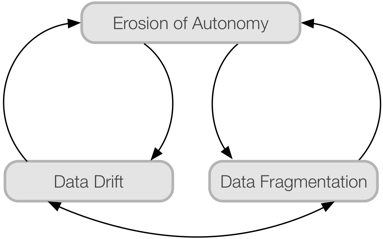
\includegraphics[scale=1.00]{figures/dbd.png}
  \caption{Cycle of Disempowerment}
  \caption*{The influence of external actors on data practices erode organizational autonomy and precipitate data drift—the altering of metrics in response to shifting requirements—and data fragmentation—the dispersal of data in non-coherent systems and schemas. These mutually-reinforcing consequences further erode autonomy leading to a cycle of disempowerment.}
  \label{fig:dbd}
\end{figure}

Autonomy of the organizations in this study is impinged upon from the start by external stakeholders---especially, but not limited to, funding agencies---whose ideas about what measurable impacts are deemed valuable implicitly or explicitly shape data practices through prescriptions of what metrics organizations should track, what information systems (owned by whom) should be used to collect M\&E data, and how such data should be reported. Data analysis is conducted by outsiders and consultants, disconnected from the organizational mission and from the organizations’ long-term vision of social impact. Data and reports are compiled in the systems of ever evolving rosters of funders, often outside the control of the organizations themselves. Taken together, these data practices eroded organizational autonomy, dictating how already over-worked staff should allocate their limited time for data practices, leading to \textit{data drift} and \textit{data fragmentation}.

This \textit{erosion of autonomy} contributes directly to \textit{data drift}---the shifting of metrics and data collection foci in response to externally re-framed missions and priorities, moving the organization towards a mission that is both undefined and unknowable. \textit{Data drift}, in turn, contributes towards an even greater erosion of organizational autonomy, as the data the organizations are left to work with moves them farther and farther away from their core mission and expertise.

The erosion of organizational autonomy also contributes to \textit{data fragmentation}---where issues of power dynamics, a reliance on external expertise and frequent stakeholder turnover lead to a proliferation of disconnected data sets. And yet, the more fragmented the data becomes, the more reliant organizations become on external expertise to fix the problem, further undermining organizational autonomy.

\textit{Data fragmentation} and \textit{data drift} are also mutually reinforcing. As the data that is collected changes over time, \textit{data drift} contributes to both longitudinal and logical fragmentation by introducing data sets that are dissimilar to previously collected data. As new types of data are collected---especially if mandated by new funders---\textit{data drift} also leads to locational fragmentation, as data is collected in or moved into new and different funder systems. Looking back the other way, \textit{data fragmentation} may also lead to \textit{data drift}, as different outside experts logically fragment data by periodically shifting focus from one set of metrics to another, resulting in a changing organizational identity as represented by their data. As the data makes less sense due to its fragmented state, the organization loses the ability to systematically understand the differences between their current and prior data environments.

These challenges compound and loop back on each other to reinforce a cycle of disempowerment overlaid on M\&E practices that are, themselves, in a near-continual state of flux. This cycle results in these organizations having an ever- decreasing role in designing their data strategy, executing their own vision, and making meaning of the data that they spend much of their constrained time collecting.

\subsection{Data Driven for Whom?}

The \textit{cycle of disempowerment} sheds new insights into the enactment and consequences of current implementations of data-driven decision making. Organizations are under great pressure to adopt data-driven decision making strategies (e.g., \cite{Haskins2011Building}). And there is some evidence, especially from the private sector, to suggest that data-driven decision making can be impactful \citep{Brynjolfsson2011Strength,Lavalle2011Big}. Yet, there are many concerns about the potential of data-driven practices in the mission-driven space, with various scholars raising possible explanations for the challenges observed: that organizations may not be adept or confident enough to use data effectively \citep{Maxwell2016Data} and that metricization is not appropriate for the mission-driven nature of organizations in this sector \citep{Benjamin2014Programs}.

What the \textit{cycle of disempowerment} foregrounds is that each of these explanations fall short of explaining why data-driven processes are not working. The M\&E professionals in mission-driven organizations are quite articulate about what kinds of data could be useful in evaluating their programs; they are invested in the work of trying to better understand how to measure impact in some of the most complex and thorny situations. Most individuals we interviewed believe that data \textit{could} be useful.

Yet, we find that the achievement of a data-driven culture is currently an impossibility—beyond the problems introduced by any particular analytics tool that thwarts the actionable use of data \citep{Verma2016DrillDown}---rooted in a more pernicious set of power relations among stakeholders. Here we find that data tools and practices are not constituting relations that newly empower organizations. Rather, data tools and practices are re-entrenching existing social relations, and making them harder to work around. Relationships with funders, for example, are being reified and reinforced through the adoption of their systems for data management---leading to increased fragmentation—and their metrics of impact and success---leading to \textit{data drift}.

This research raises the question of “data-driven for whom?” The acute political imbalance that disempowers the organization and its own expertise suggests broader implications about what may be happening more or less invisibly in so-called successful exemplars of data practices (e.g., \cite{Brynjolfsson2011Strength,Lavalle2011Big}). If data practices serve those who make decisions about what data to collect and how to collect it, and definitions of success shift to align with the metrics that are measured, the positive outcomes of data-driven decision making risk being self-reinforcing. Researchers are beginning to key in on the fact that certain metrics are being over-reified in ways that re-define what constitutes success, especially in health settings \citep{Pine2015Politics,Pine2015Emerging}. As the construction of health becomes tightly bound up in particular metrics—--e.g., heart rate, blood pressure—then interventions in response to changes in those metrics will always appear to result in better health outcomes. Yet, if health was understood in other terms, then acting on the data that these metrics offer---striving to keep heart rate or blood pressure within a certain target range while ignoring other effects---may \textit{not}, in fact, produce positive outcomes for patients.

Given the \textit{cycle of disempowerment} in mission-driven organizations, we are concerned that their \textit{data drift} might move organizations towards increasing alignment with metrics about the health of their programs and services that stand to be similarly self-reinforcing—that organizations will appear to be more ‘successful’ over time as they abandon and re-shape their mission to the terms of the data at hand. This is the pernicious consequence of \textit{data drift}, that it changes the potential futures that the organization might have. It also changes the potential futures for those clients, constituents, and beneficiaries served by the organization.

\subsection{Disempowered at Whose Expense?}

What is strikingly absent from the data in this research are discussions about the role of client, constituent, and beneficiary feedback in the evaluation work of mission- driven organizations. This absence is particularly striking because the preponderance of mission-driven organizations provide direct products and services to individuals who are, themselves, already marginalized. The only instance in this research of M\&E professionals discussing constituent feedback in their work practice emerged from a participant reflecting on the lack of constituent feedback, which she attributes to challenges in technology adoption. While P3 believes that there are appropriate tools available to help organizations collect constituent feedback, in her view, “...the problem is adoption. How do we get people [organizations] to care about this and use these tools?” (P3)

There is ample evidence in the HCI literature about adoption challenges that derive from inequalities between who does the work and who benefits \citep{Grudin1994Groupware}, and this likely plays a role. However, our research suggests that the non-use of tools that would support constituent data collection is not simply a lack of \textit{caring}. Our research suggests that the disempowerment of clients, constituents, and beneficiaries---through not having a voice in the M\&E practices of mission-driven organizations---is likely a result of the disempowerment of the mission-driven organizations, themselves: staff pressured to navigate a complicated web of actors that perpetuate a cacophony of data demands, drawing them away from the centrality of their mission as embodied by and through constituents. As M\&E work becomes further institutionalized and as metrics for evaluation stand to become standardized in the infrastructures of organizations and their funders, this is the time for calling out the disempowerment of clients, constituents, and beneficiaries at the hands of externally prescribed data practices.

\subsection{Designing to Disrupt the Cycle of Disempowerment}

In the early 1800s, statisticians from the French Bureau de Statistique undertook one of the first comprehensive national censuses, sending questionnaires to each départment \citep{Porter1995Trust}. Yet the Bureau “quickly learned that no single set of categories could be adequate” and asked local authorities to supplement the national census categories with locally- defined categories. As Porter writes, drawing on Bourget’s earlier work, “‘recognizing the existence of a diverse, local reality, irreducible to the categories of a national accounting’ was a damaging concession” to the viability of a purely nationally framed census (\cite{Porter1995Trust} quoting Bourguet).

The tensions between uniform metrics and the metrics that derive from and reflect local experience, then, are not a new problem. Yet as evidenced by the recent surge in scholarship on this topic at CHI and CSCW, it remains a thorny problem for researchers to figure out how to address in new ways \citep{Bowker2000Sorting,Pine2015Politics,Voida2017Currencies,Verma2016DrillDown}. Through our study of the work practices of M\&E professionals, we see quite distinctly the negative organizational outcomes of these tensions being resolved---as is currently—without sufficient local input. Any disruption of the \textit{cycle of disempowerment} is likely to require granting some autonomy in data practices to organizations. And yet, disrupting the cycle would require disrupting entrenched relationships among funders, organizations, ratings agencies, and others, as power is constituted through these relationships. But what researchers can do is tell stories about data practices and their presumably unintended consequences on organizations. Researchers can convene groups of stakeholders for participatory design workshops to engage in dialogue about data and undertake collaborative processes of commensuration (see \autoref{ch:wkshp}).

But we also see a critical role for researchers and designers in designing new data systems that help individuals and organizations work around imperfect and incomplete data. The design of information systems used in the mission- driven sector nearly always lock organizations into fixed schemas and demand a complete year-on-year set of data. Nearly all M\&E professionals who participated in this research believed that imperfect or incomplete data was generally useless for developing a longitudinal or comprehensive analysis of social impact. But whether the data collected and managed evolved through \textit{data drift} or through evolving understandings of what metrics were important to capture, nearly all organizations in this study reported changes to their data over time. And surely there is a broader design space worth exploring for supporting evidenced-based research about social impact without over proscribing the mathematization of ‘data’ or requiring perfect statistical inputs. What would it look like to build data systems from a sociological or historical perspective, for example? What would it look like to build data systems that drew on tools of interpretivist traditions that might not require psychological or mathematical ideals of explanation to enable M\&E professionals be able to learn things useful about the work of their organization?

\subsection{A Note About Our Use of Disempowerment}
Although our analysis of data from interviews with M\&E professionals suggests that these organizations are currently caught in a \textit{cycle of disempowerment}, we do \underline{not} see any evidence that these organizations should be relegated to a permanently marginalized standing with respect to data. And indeed, scholarship in community-based research warns against labeling communities as “damaged,” as these labels stand to further contribute to marginalization and disempowerment \citep{Tuck2009Suspending}. We do not intend to suggest that mission-driven organizations or other stakeholders discussed in this paper are damaged. Indeed, the M\&E professionals who participated in this research have significant expertise and it is essential to find ways that this expertise can be given the weight it deserves. Our intent, then, is to draw attention to the cycle so that we are better able to move beyond it.

\section{Conclusion}
In the context of monitoring and evaluation, where the role of data stands to be most tightly aligned with the mission of the organization and the passion of its employees, data practices are all-too-often experienced as busy work. For the participants in this research, data practices are predominantly experienced as a production for others that might happen at scale, but that is disconnected from any localized meaning or value and isolated from the complexities of the social situations these organizations operate within.

Mission-driven organizations serve critical social roles. However, the disempowerment of organizations in this study suggests that the cards are stacked against the very organizations that our communities rely upon. As staff get caught up in the demands of data practices, autonomy is eroded, data is fragmented, and the organization begins to change through \textit{data drift}. These consequences come together to result in organizations that are neither empowered nor equipped to think and plan for the long term, despite our communities’ needs for such strategic planning.

In this research, we have made the following contributions:
\begin{enumerate}
	\item Provided an empirical account of the data practices of monitoring and evaluation professionals in mission-driven organizations;
	\item Identified three negative consequences of current monitoring and evaluation practices: \textit{erosion of autonomy, data drift,} and \textit{data fragmentation;} and
	\item Identified relationships among these consequences, demonstrating how they collectively reinforce a \textit{cycle of disempowerment} for the mission-driven organization.
\end{enumerate}

There is promise for the role of data in the monitoring and evaluation work of mission-driven organizations. Yet, this study of data practices demonstrates that this empowering use of data is currently thwarted. Now—at this opportune cusp when new practices are starting to collide with the new-to-data-driven-decision-making value orientations of the mission-driven sector—is the time for intervening in ways that might support and empower mission-driven organizations in their use of data.






















